\documentclass{mcmthesis}
\mcmsetup{CTeX = false,   % 使用 CTeX 套装时,设置为 true
        tcn = 55869, problem =  C,
        sheet = true, titleinsheet = true, keywordsinsheet = true,
        titlepage = false, abstract = true}
\problem{C}

\makeatletter % `@' now normal "letter"   %follpw as section test
\@addtoreset{equation}{section}
\makeatother  % `@' is restored as "non-letter"
\renewcommand\theequation{\oldstylenums{\thesection}%
                   .\oldstylenums{\arabic{equation}}}

\usepackage{palatino}
\usepackage{mwe}
\usepackage{graphicx}
\usepackage{tabularx}
\usepackage{float}
\usepackage{indentfirst}
\usepackage{amsmath}
\usepackage{caption}
\usepackage{subfigure}
\title{}
\date{}

\begin{document}

\begin{abstract}%摘要


\title{Keep the Bathtub Warm}



\end{abstract}

\begin{keywords}
	\textbf{A,\indent B, \indent}
\end{keywords}
\maketitle
\tableofcontents\thispagestyle{empty}
%设置页眉
\newpage

\setcounter{page}{1}
%Section 1
\section{Introduction}

\section{Assumptions}
\noindent
{\bf (1) } \textbf{example.} example.\\

\section{Symbol Description}
\begin{table}[H]
        \setlength{\abovecaptionskip}{0pt}
        \setlength{\belowcaptionskip}{0pt}
				\centering{Table 1:Constants}\\
        \begin{tabular}{p{2cm}|p{2cm}|p{7.5cm}|p{1.7cm}}
		\hline
		\rowcolor[gray]{0.9}\bf{Symbol}	&\bf{uint}      &\bf{Meaning}&\bf{value}	\\
		\hline
		${P}''_{v}$		& $hP_{a}$		 & example  &12\\

		\hline
		\end{tabular}
	\end{table}

\begin{table}[H]
        \setlength{\abovecaptionskip}{0pt}
        \setlength{\belowcaptionskip}{0pt}
        \centering{Table 2:Notation} \\
        \begin{tabular}{p{1.8cm}|p{2.2cm}|p{9cm}}
        \hline
        \rowcolor[gray]{0.9}\bf{Symbol}	&\bf{uint}      &\bf{Meaning}\\
        \hline
        $V(h)$			& $m^3  $		 & example \\
        \end{tabular}
        \end{table}

%Section 3
\section{Heat Dissipation Model}
example
\begin{equation}
\begin{split}
h=H(v)  \\
S_{1}=S_{1}(h) \\
S_{2}=S_{2}(h)  \\
\end{split}
\end{equation}
\indent example\\
\begin{itemize}
\item{Liquid surface heat loss model.\\ }
\item{contact area of liquid and bathtub heat loss model.\\ }
\end{itemize}



\section{Model of Hot Water Addition}

\subsection{example}
 
\begin{figure}[H]
\centering
\subfigure[When Kp is too small]{
\begin{minipage}{7cm}
\centering 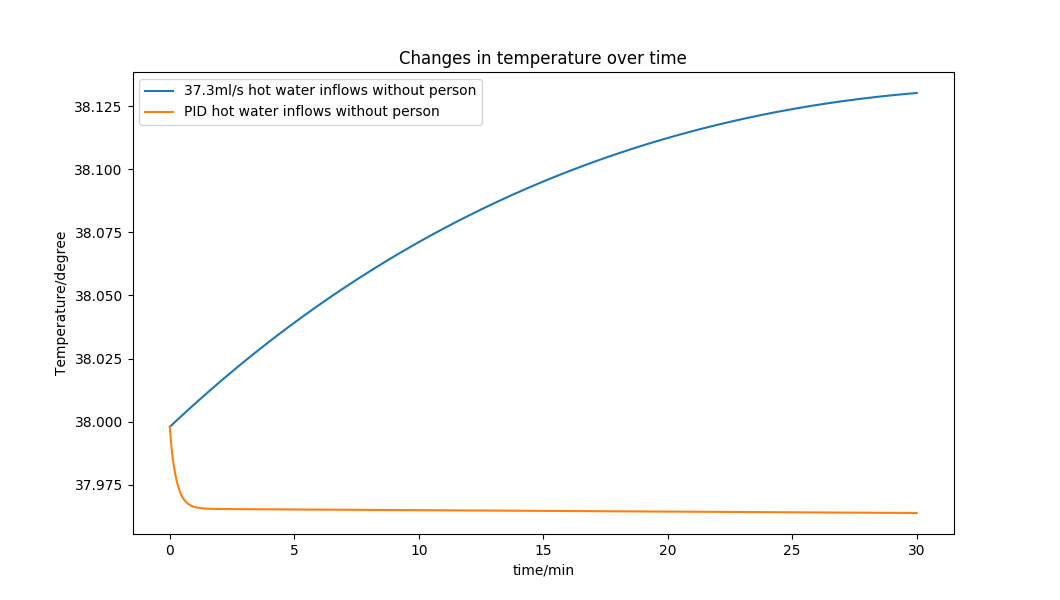
\includegraphics[scale=0.26]{PID_1.png}       
\end{minipage}
}
\subfigure[When Kp is too large]{
\begin{minipage}{7cm}
\centering                                    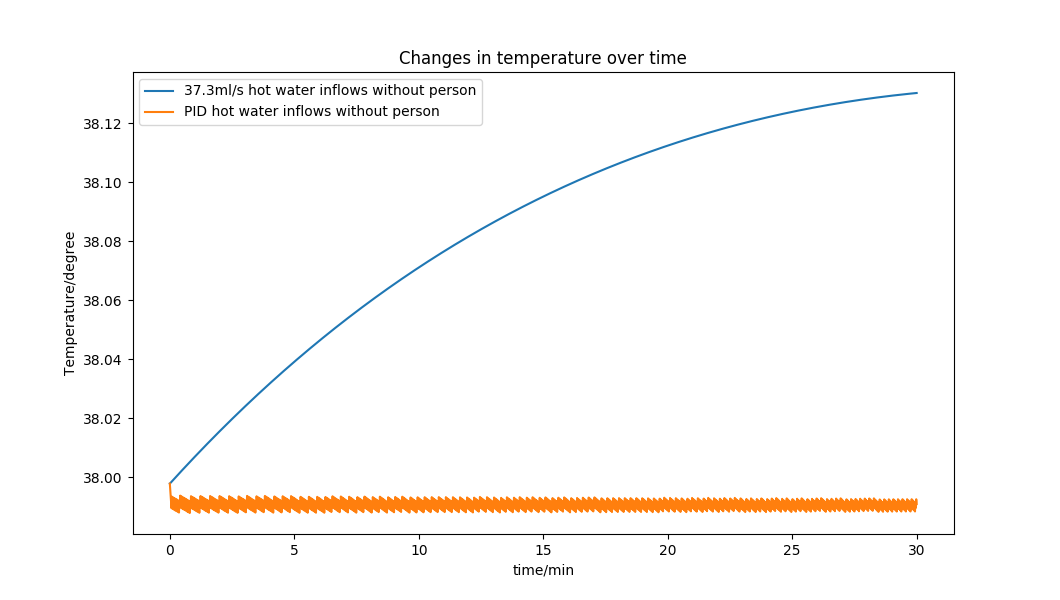
\includegraphics[scale=0.26]{PID_4.png}        
\end{minipage}
}
\caption{Only use Kp}
\label{PID1}
\end{figure}



\section{Strengths and Weaknesses}



\section{References}
\begin{thebibliography}{99}
\bibitem{1}Zhenguo Zhao. Formula of enthalpy difference for water surface heat dissipation and its application[J]. Journal of Hydraulic Engineering, 2004(02):34-38.

\end{thebibliography}



\end{document}